\chapter{Aufbau \sppname}

\section{Architekturbeschreibung}
\label{sec:spp_arch}

Sinn und Zweck des \gls{snort} \gls{praeprozessor}s \gls{sppname} ist das Abfangen,
Komprimieren und Weiterleiten von \gls{profinet}-\glspl{paket}n. Diese
sind durch den \gls{ethertype} unterscheidbar. Zur Einführung des Programms wird der Präprozessor ausschließlich \glspl{paket} mit dem Ethertyp 0x8892 behandeln, welcher die Realtime Kommunikation von Profinet identifiziert.

Hauptbestandteil des \gls{praeprozessor}s ist eine erweiterbare Baumstruktur von Decodern, welche rekursiv, Schicht für Schicht, ein \gls{paket} bearbeiten und benötigte Informationen in einer Protokollbaum Struktur ablegen. Aus dem Protokollbaum (ProtocolTree) wird schließlich ein \gls{truffle} mit den von \gls{programname} verwendeten Informationen erstellt. Ein \gls{truffle} ist eine durch den \gls{praeprozessor} definierte Datenstruktur.
Pro Netzwerk-\gls{paket} entsteht ein \gls{truffle}, welches erheblich kleiner und kompakter als herkömmliche Netzwerkpakete ist. Das Truffle wird über die Serververbindung des {praeprozessor}s an \gls{programname} versendet (Sender). Die klar definierte Truffle Struktur ermöglicht einerseits einen geringeren Overhead bei der Übermittlung der Paketdaten (anstelle des gesamten Pakets) und gewährt zusätzlich einen Gewinn an Sicherheit. Durch das bewusste einfügen von Informationen des Pakets am Ende der Dissektion in die Trufflestruktur vermeidet man, dass falsch (auch vorsätzlich falsch) definierte Daten versehentlich als echte Information zum Client gesendet werden. Ab diesem Zeitpunkt kann somit für mehr Sicherheit im Informationsfluss gesorgt werden.
Ein weiterer Vorteil der \glspl{truffle} Struktur ist die Gelegenheit für einen Sicherheitscheck bevor es gesendet wird. Aufgrund der rekursiven Struktur des Decoder-Baums ist immer ersichtlich welche Daten zu erwarten sind. Sollten Inkonsistenzen festgestellt werden bzw. Fehler vorliegen werden im Truffle entsprechende Flags gesetzt, damit \gls{programname} Statistiken für Auffälligkeiten einzelner Kommunikationsteilnehmer angefertigt werden können.\newline

\section{UML-Diagramm}

\begin{sidewaysfigure}
  \centering
  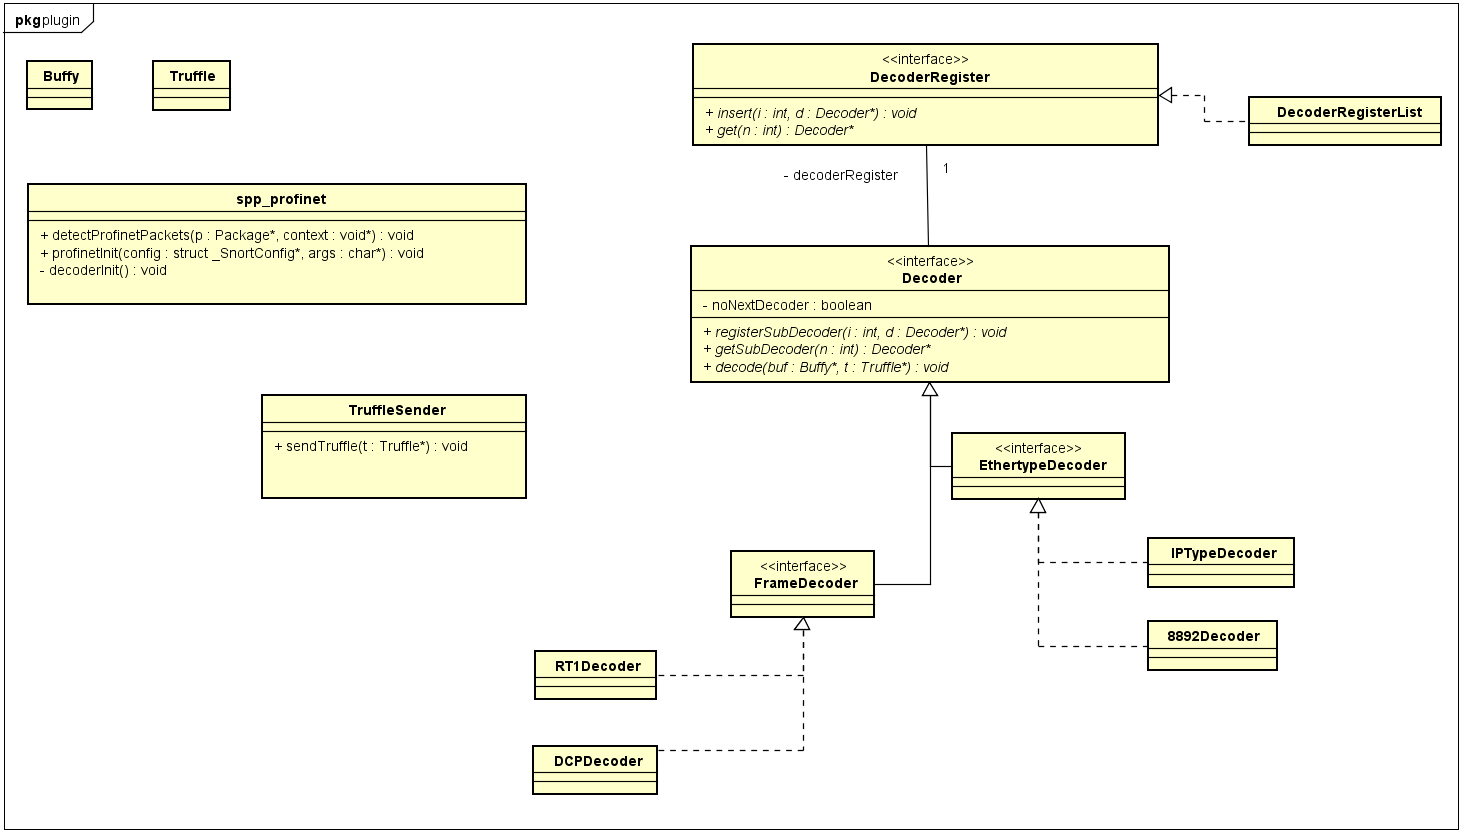
\includegraphics[width=\paperwidth]{../diagramimages/spp_profinet.png}
  \caption{\gls{praeprozessor} \gls{sppname}}
  \label{fig:spp_uml}
\end{sidewaysfigure}
